%\part{Aspectos Gerais}

\chapter[Referencial Teórico]{Referencial teórico}
	
	Este capítulo tem como objetivo servir como referencial teórico para todo o documento. As idéias discutidas neste capítulo são
	
\section{Qualidade}
	O principal produto da engenharia de software é o software, contudo o que tem se vivenciado na realidade brasileira de computação é que o software que está sendo entregue é um software precário e de baixa qualidade. Por ser uma palavra abstrata, o conceito de qualidade é bem amplo, porém o termo qualidade normalmente está associado a uma medida relativa, essa qualidade pode ser entendida como "conformidade às especificações". Conceituando dessa forma, a não conformidade às especificação é igual a ausência de qualidade \cite{Paduelli}.
\\ A ISO 9126-1 descreve o modelo de qualidade voltado para o produto de software como sendo composto por duas categorias como pode ser visto na Figura \ref{img:relacao_iso}. A primeira categoria está relacionada a qualidade interna e a qualidade externa do software. A segunda categoria se relaciona com a qualidade de uso do software \cite{_nbr_2016}
\graphicspath{{figuras/}}
\begin{figure}
\centering
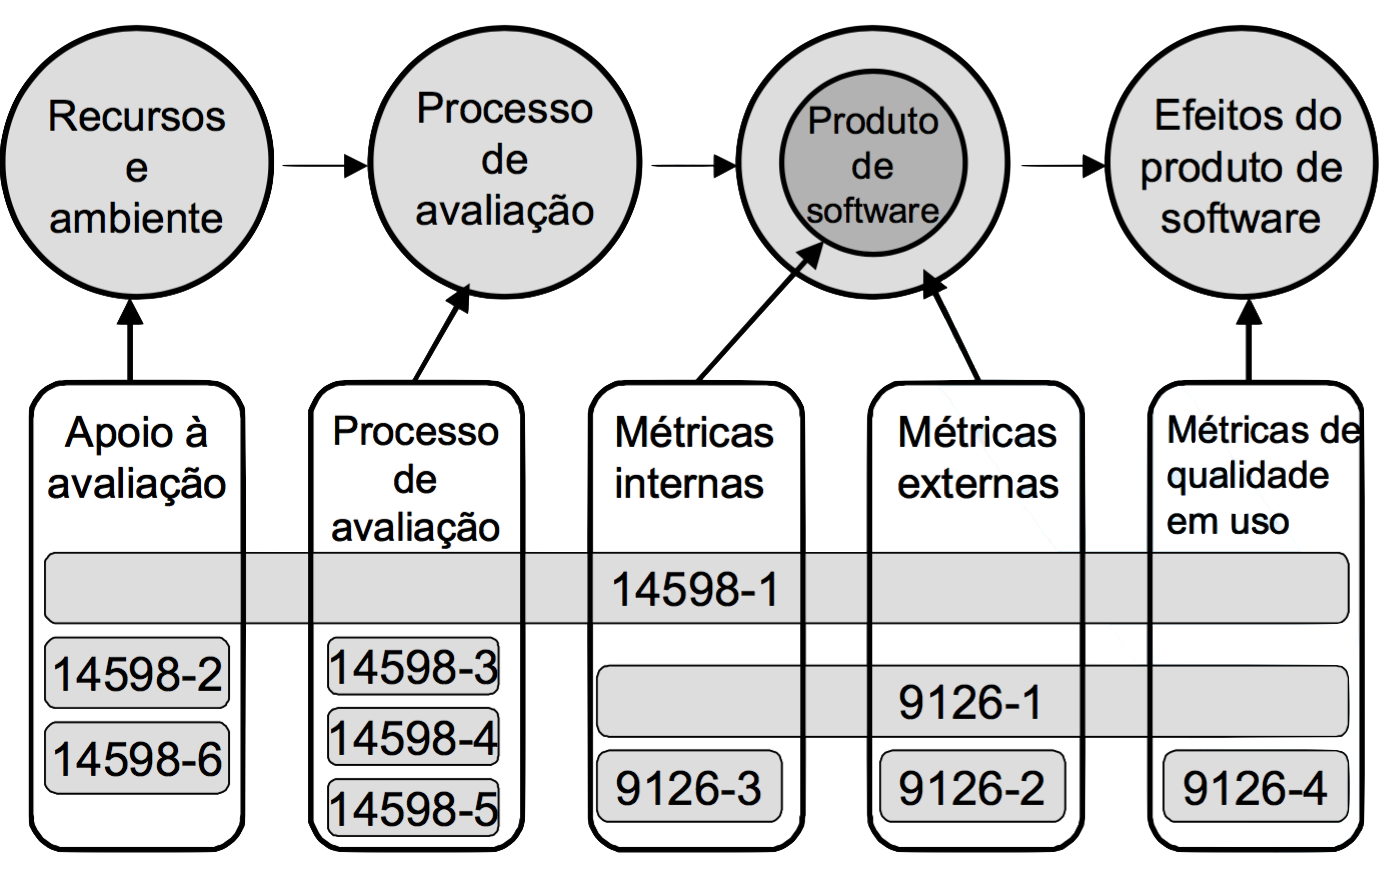
\includegraphics[scale=0.40]{ISO}
\caption{Relação entre as NBR ISO/IEC 9126 e NBR ISO/IEC 14598 .Fonte:\cite{_nbr_2016}}
\label{img:relacao_iso}
\end{figure}
\\ Sob o aspecto de modelo de qualidade, a qualidade interna do produto de software é vista como sendo o somatório das características do ponto de vista interno. Os principais produtos desta categoria são os de cunho intermediário, dentre eles: relatórios de analise estática do código fonte, revisão dos documentos produzidos, entre outros. A qualidade externa por sua vez já apresenta o seu foco mais voltado para as relações externas do software, normalmente esta relacionado com a execução do código coletando suas métricas enquanto o software está em funcionamento. A Figura \ref{img:modelo_qualidade} apresenta a divisão proposta pela \cite{_nbr_2016} onde são categorizados seis aspectos de qualidade de software e suas subcaracterísticas, essas podem ser medidas por meio de métricas internas e externas. 
 \graphicspath{{figuras/}}
\begin{figure}
\centering
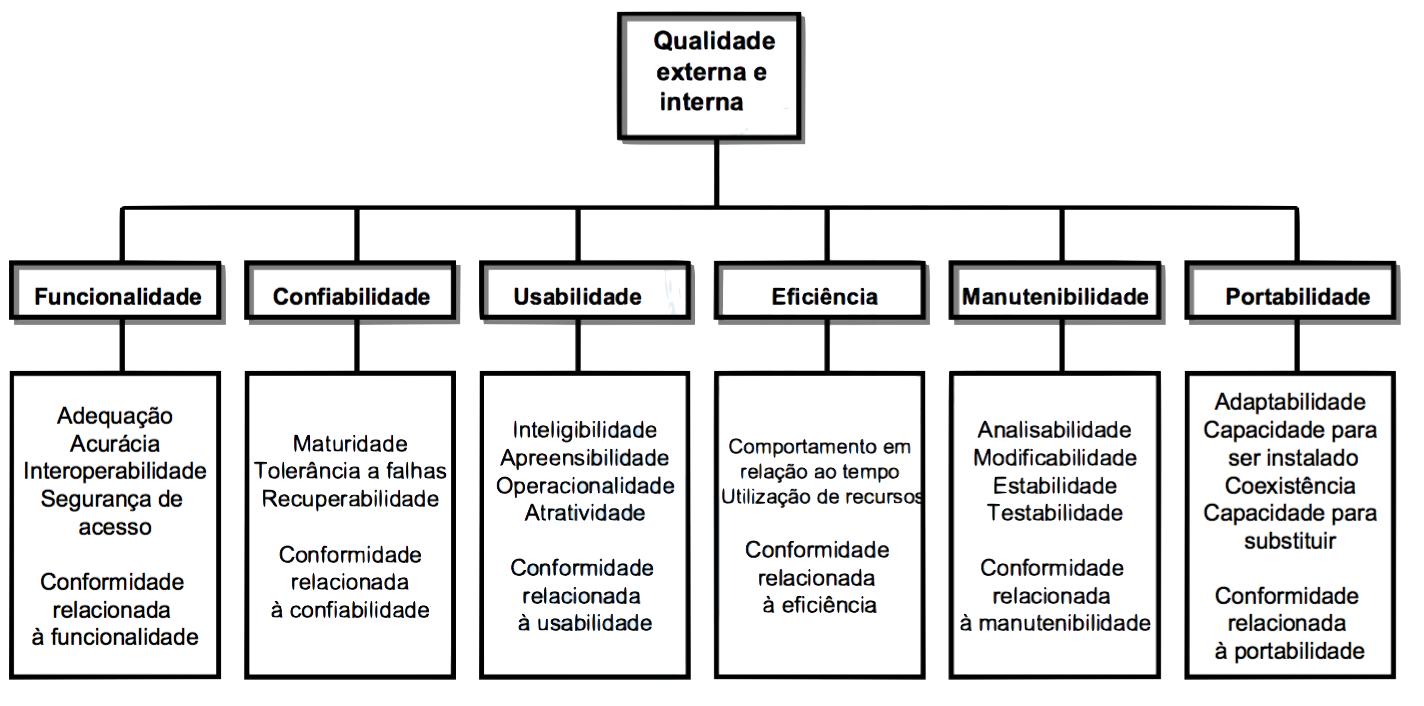
\includegraphics[scale=0.50]{Modelo_de_Qualidade}
\caption{Modelo de Qualidade para Qualidade Interna e Externa .Fonte:\cite{_nbr_2016}}
\label{img:modelo_qualidade}
\end{figure}
 